\section{The FP420 Project} \label{fp420}

FP420 is a proposed new sub-detector capable of measuring the momenta of the protons scattered in central exclusive processes \cite{Cox:2005tb}. The basic design of FP420 is a magnetic spectrometer. The protons scattered during the interaction will have lower momentum than the beam protons and will be bent out of the beam by the superconducting magnets in the LHC ring. The aim is to install movable silicon tracking detectors 420~m either side of the interaction point. The measurement of the angle and displacement of the protons with respect to the beam line will allow the proton momentum to be determined if the beam optics are well known.%large dispersion at 420

In the present design of the LHC, there is a 15~m connection cryostat in the 420~m region. The cross section of the cryostat is shown in figure \ref{cryostat420}. V1 and V2 are the beam pipes, with V2 containing the outgoing beam from the interaction point. The detector stations will be placed between V1 and V2. M1, M2 and M3 are superconducting bus bars which carry the current for the magnets. It is possible to move these bus bars to make extra room for detector access. 
%A possible re-design of the cryostat region is shown in figure \ref{cryostat420} (b). The region marked XX would contain the bus bars. 
The heat exchanger, labelled $X$, cannot be moved because it must remain parallel to the tunnel floor at all times. 
%this bit is about the cold bit.......do i need it?
%The 420m region is a `cold' region which means that the beam pipes are at 1.9K. The FP420 design will, point::::::> no longer a cryo!!!!!!

\begin{figure} [t]
\centering
    	\includegraphics[width=0.65\textwidth]{Diagrams/Cryostat.eps}
\caption[The 15~m cryostat at 420~m from the ATLAS interaction point]{The 15~m cryostat at 420~m from the ATLAS interaction point \cite{Cox:2005tb}.\label{cryostat420}}
\end{figure}

%check this next bit %prev say that two sets of detectors 8m apart ??
The detector stations will be moved closer to the beam after proton injection and acceleration, when the beam has stabilised. 
%delete this if incorrect.........
The Hamburg Pipe design proposes that the stations will be rigidly fixed to the V2 beam pipe and the position measured to 1~$\mu$m with an optical bench arrangement. The entire structure will then be moved to place the detectors closer to the beam line itself. 
%
%
The position of each station with respect to the beam will be measured using beam positioning monitors (BPMs), which are precise to a few 10's of $\mu$m. %A greater precision can be achieved using a known high-rate process 
At least two detector stations will be required to make the momentum measurement, but 3-4 could be used for redundancy purposes and background (halo) rejection. The stations will be placed over an 8~m length along the beam pipe.

%some citations needed here.......
Each detector station will be capable of measuring the position of the proton relative to the beam and the time of flight (TOF) of the proton from the interaction point.
The position measurement will be made using layers of 3D edgeless silicon. It is estimated that the position of a proton hit within the silicon layers can be measured to 10~$\mu$m and the angle to 1-2 mrad \cite{Cox:2005tb}. The limiting factor on the relative position measurement will be due to the BPMs and this can probably be improved using clean high rate processes such as $\gamma \gamma \rightarrow \mu^{+} \mu^{-}$ in off-line calibration.

The TOF detectors will be fast-timing Cerenkov counters. Protons traversing the active volume will emit Cerenkov radiation which is then detected by photo-multiplier tubes. Two types of TOF unit will be used; GASTOF and QUARTIC, which are designed to use gas and quartz respectively. GASTOF will be used in the stations nearest the interaction point whilst QUARTIC will be used only in the final station and will be positioned after the silicon layers. This configuration was chosen because there will be a large probability for the proton to have multiple scatterings in  quartz, which could change the direction of the proton or cause it to break up completely. Thus QUARTIC can only be used after all of the position measurements.
The final TOF measurement is estimated to be accurate to 10~ps. The TOF measurements for the outgoing protons either side of the interaction point will be made relative to each other, making a reference clock unnecessary. The $\Delta$TOF measurement
corresponds to an interaction vertex measurement with an accuracy of 2.1~mm.

The $\xi$ acceptance will depend upon how close the detector stations can get to the beam and the dispersion of the LHC at 420~m. The closest distance of approach to the beam has been considered to be 10$\sigma_x + 0.5$~mm \cite{Alekhin:2005dy:TOTEM},
where $\sigma_x$ is the horizontal beam width at 420~m. This results in a lower limit of 3~mm and will require ideal beam conditions. Larger distances of 5~mm, 7.5~mm and 10~mm have also been studied \cite{Cox:2005tb}. The distance from the beam will affect the low $\xi$ acceptance, and hence the lower central mass reach of FP420. However, using the FPTRACK program \cite{PeterBusseyAcceptance}, it was found that the acceptance for a 120~GeV central mass is constant for the three closest configurations as shown in figure \ref{fp420accept}. The $\xi$ acceptance of the 5~mm configuration is given \cite{PeterBusseyAcceptance} by %PB
\begin{eqnarray}
0.0023 & \leq \xi_1 \leq & 0.0129 \nonumber \\
0.0029 & \leq \xi_2 \leq & 0.0171 
\end{eqnarray}
where the asymmetry is due to differences in the beam optics on each side of the ATLAS detector. The dominant contribution to the uncertainty in the momentum loss measurement is expected to be the intrinsic momentum spread of the protons within the beam at the LHC (0.77~GeV). This is also the dominant uncertainty on the resolution on the central mass measurement, which is estimated to be $1-2\%$. 

\begin{figure} [t]
\centering
    	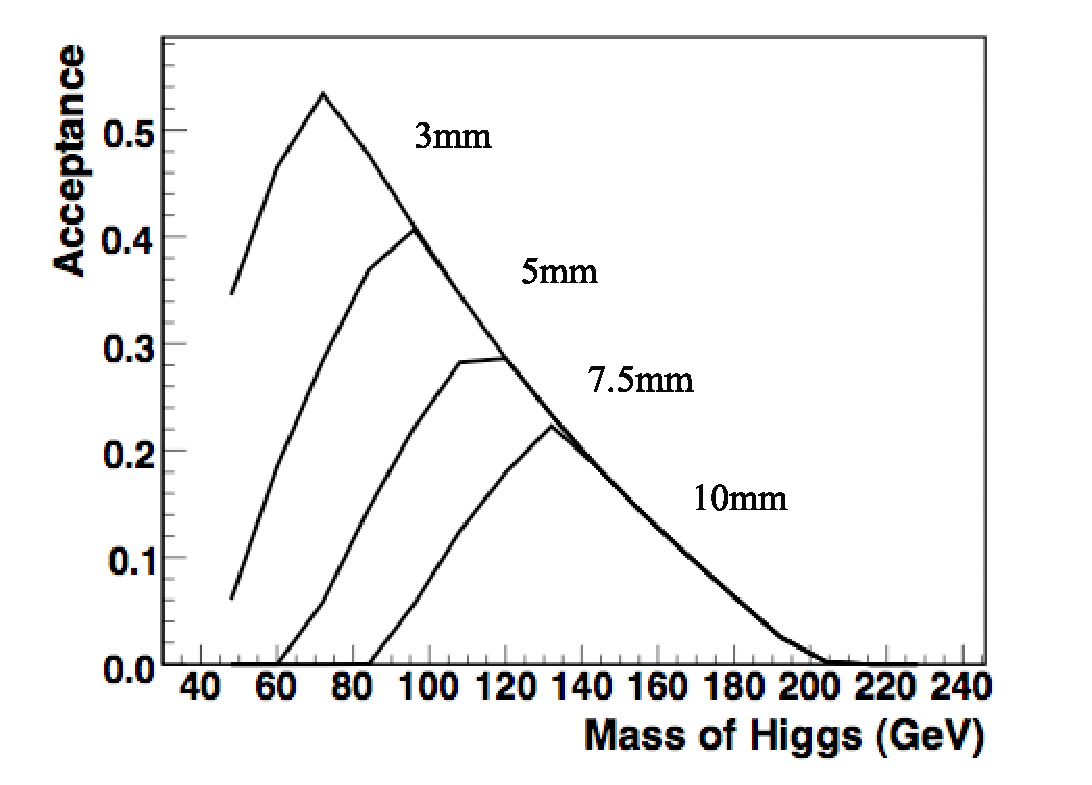
\includegraphics[width=0.65\textwidth]{Diagrams/peterbusseyacceptance.eps}
\caption[The acceptance of FP420 as a function of the mass of the central system]{The acceptance of FP420 \cite{Cox:2005tb} as a function of the mass of the central system. Results are shown for different distances of closest approach to the beam.\label{fp420accept}}
\end{figure}

Finally, the signal from FP420 will arrive at the central trigger processor 3~$\mu$s after the interaction occurred. This means that information from FP420  can only be used at trigger level 2 onwards. Thus the central exclusive events will only be available for analysis if they pass one of the standard level 1 triggers given in section \ref{triggers}.
